\chapter{Geladenes Teilchen im elektrischen Feld\label{chapter:efeld}}
\lhead{Teilchen im elektrischen Feld}
\begin{refsection}
\chapterauthor{Michael Cerny und Stefan Schindler}

\index{Potentialkasten!Anwendung}


In diesem Kapitel erweitern wir das Beispiel des Potentialkastens 
(Kapitel \ref{subsection:potentialkasten}, Seite \pageref{subsection:potentialkasten})
um eine St\"orung.

\section{Grundlagen St"orungstheorie}
Grunds"atzlich k"onnen wir mit der St\"orungstheorie ein einfaches Modell 
(Abb \ref{abb:efeld_psi_ungestoert} der ersten 5 Energieniveaus) 
mit einer St\"orung erg"anzen, statt von Anfang an mit einem komplexen Modell zu rechnen.

\begin{comment} %fixme
\[
  f(x, \varepsilon) = f_0(x) + \varepsilon^1 f_0(x) + \varepsilon^2 f_0(x) + \ldots
\]
\[
  |\psi_n(\varepsilon)\rangle =
  |\psi_n^{(0)}(\varepsilon)\rangle + \varepsilon^1 |\psi_n^{(1)}(\varepsilon)\rangle
  + \varepsilon^2 |\psi_n^{(2)}(\varepsilon)\rangle + \ldots
\]
Wir betrachten in unserer Anwendung nur die erste N\"aherung
und werten deshalb nur die Terme mit den Indizes $0$ und $1$ aus.
\end{comment}

F"ur die erste N"aherung gilt:
\[
  f(x, \varepsilon) = f_0(x) + \varepsilon f_1(x)
\]
Dabei ist $f_0(x)$ die ungest"orte Funktion und $\varepsilon f_1(x)$ die St"orung.
$\varepsilon$ ist eine Variable mit der wir den St"orungsterm $f_1(x)$ steuern.
Dabei sollte $\varepsilon$ nicht zu gross gew"ahlt werden,
da die N"aherung sonst ungenau wird.
Setzen wir hingegen $\varepsilon = 0$, k\"onnen wir die St"orung dynamisch abschalten.




In der Quantenmechanik k"onnen wir die St"orungstheorie anwenden,
indem wir den Hamilton-Operator der urspr"unglichen Funktion $H_0$
um $\varepsilon H_1$ erg"anzen:
\[
  H = H_0 + \varepsilon H_1.
\]

Indem wir die Energie und die Wellenfunktion der St"orung berechnen, k"onnen wir das gest"orte System ganz einfach beschreiben:
\begin{equation}
\begin{aligned}
E_k(\varepsilon)&=E_k^{(0)} + \varepsilon E_k^{(1)}
\\
\psi_k(\varepsilon)&=\psi_k^{(0)} + \varepsilon \psi_k^{(1)}
\end{aligned}
\end{equation}

Ein grosser Vorteil dabei ist,
dass wir die St"orungsterme $E_k^{(1)}$ und $\psi_k^{(1)}$
direkt aus dem ungest"ortem System berechnen k"onnen,
ohne nochmals die Schr"odingergleichung l"osen zu m"ussen.
Wir m"ussen also f"ur die erste N"aherung nur $E_k^{(0)}$,
$\psi_k^{(0)}$ und $\varepsilon$ kennen.




\section{Potentialkasten mit elektrischem Feld}

\subsection{Ausgangslage}

\begin{figure}
 \centering
 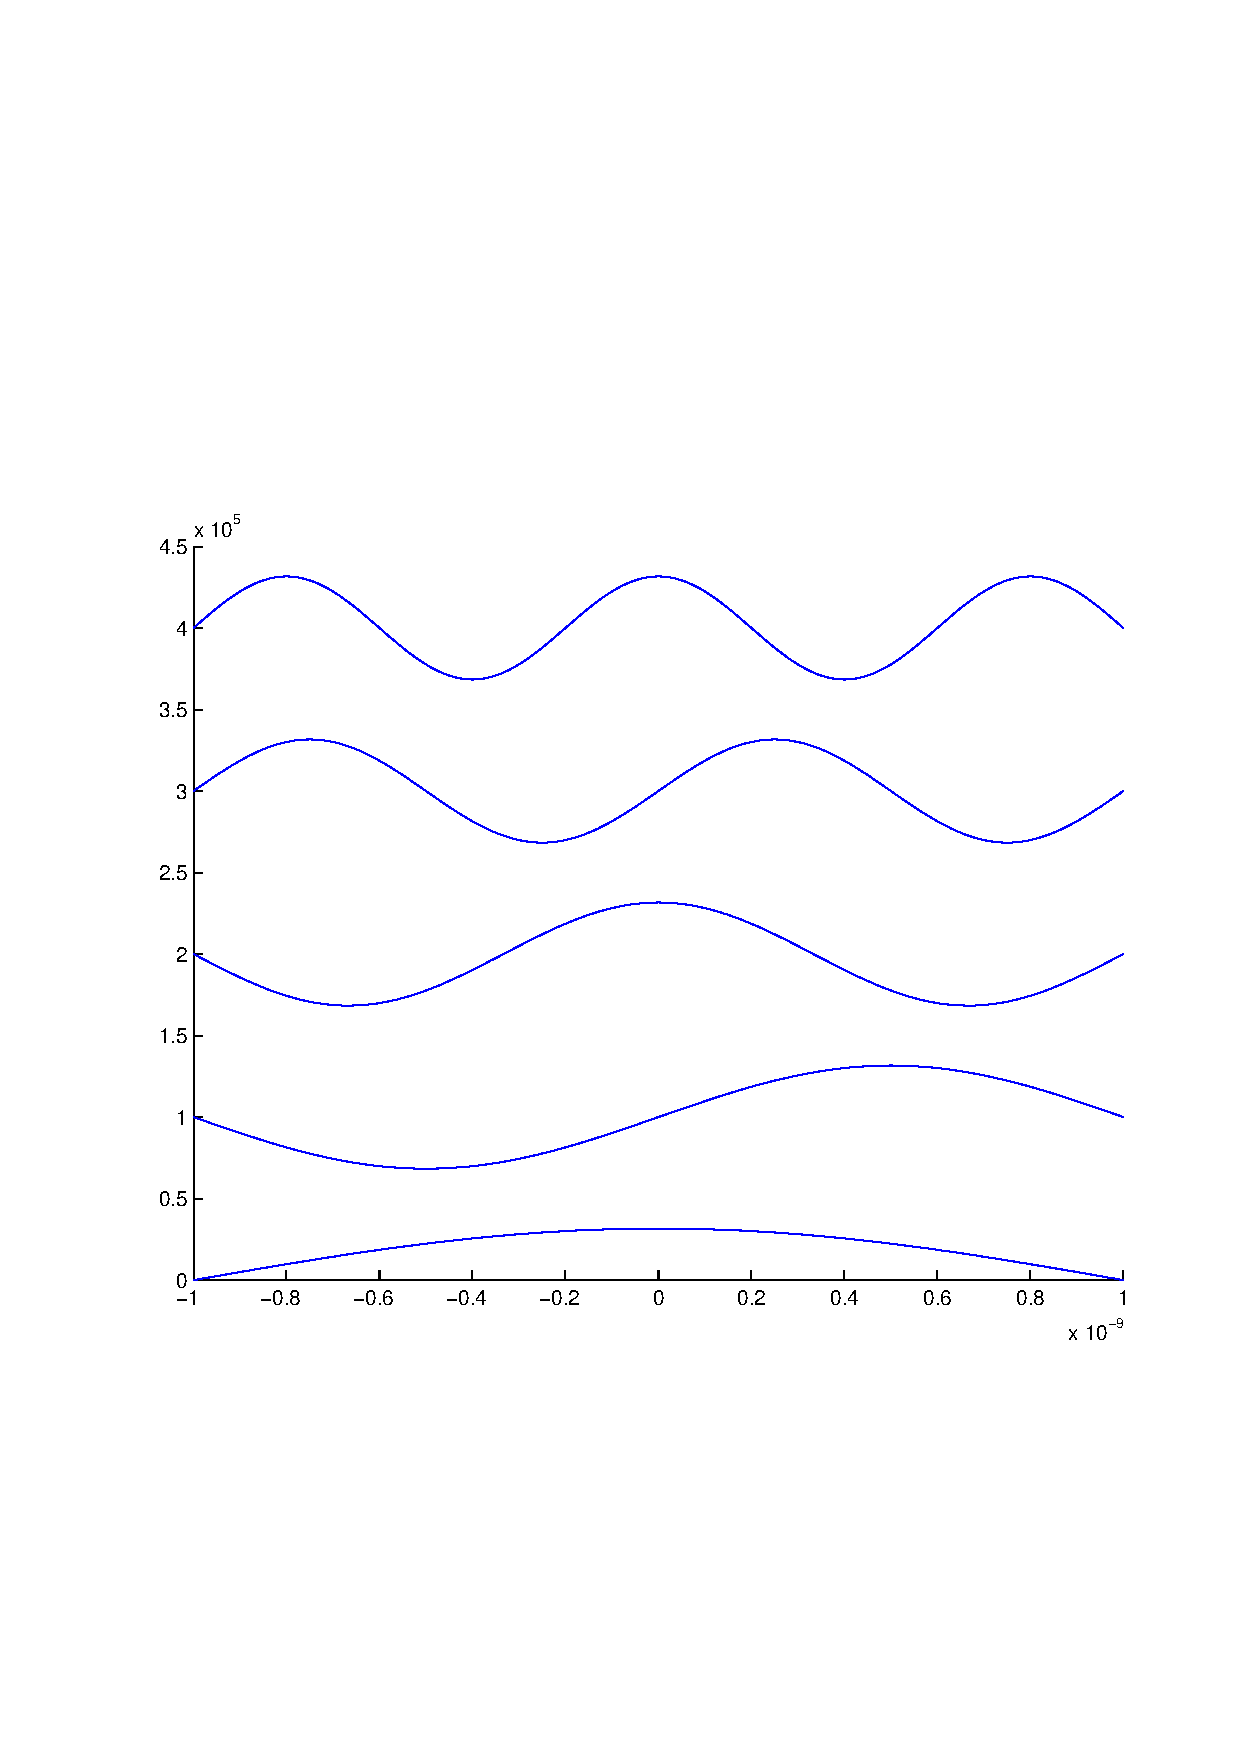
\includegraphics[width=12cm,clip=true,trim=2cm 7cm 1cm 8cm]{efeld/Psi_ungestoert.pdf}
 \caption{$\psi_k^{(0)}$ - Die ersten f\"unf ungest\"orten Energieniveaus von $H_0$ }
 \label{abb:efeld_psi_ungestoert}
\end{figure}

Bei unserer Anwendung bauen wir auf dem Potentialkasten (Kapitel \ref{subsection:potentialkasten}, Seite \pageref{subsection:potentialkasten}) auf.

Dabei geht es um ein Elektron welches zwischen zwei Barrieren mit unendlich hohem Potential gefangen ist.
Zwischen den Barrieren kann sich das Teilchen mit den Wellenfunktionen $\psi_k$
% FIXME E_k fehlt
\begin{align}
\psi_k(x)
&=
\begin{cases}
\displaystyle
\frac{1}{\sqrt{l}}\cos\frac{k \pi x}{2l}&\qquad \text{$k$ ungerade}\\
\\
\displaystyle
\frac{1}{\sqrt{l}}\sin\frac{k \pi x}{2l}&\qquad \text{$k$ gerade}.
\end{cases}
\end{align}
bewegen.

Die Gleichung wird bei (\ref{skript:potentialkasten-psi-normiert}) Seite \pageref{skript:potentialkasten-psi-normiert} erkl"art.
Ausserhalb des Potenzialkastens kommt das Elektron nicht vor.

Wir legen jetzt eine Spannung "uber dem Potentialkasten an
und erweitern so das System mit einer St"orung.

Weil das Elektron eine negative Ladung besitzt ver"andert sich seine Wellenfunktion.

Als Grundlagen verwenden wir die Hamiltonfunktion und das Potential des Teilchens im Potentialkasten
% FIXME was sagen diese Funktionen?
\begin{equation}
\begin{aligned}
H_0&=\frac1{2m}p^2+V_0(x)
\\
V_0(x)&=
  \begin{cases}
    0       & \qquad |x|<l\\
    \infty  & \qquad\text{sonst}
  \end{cases}
\end{aligned}
\end{equation}
und erweitern sie mit der St"orung $H_1$ (Abbildung \ref{abb:efeld_H_1}), welche wir als lineares 
Potential definieren:
\begin{equation}
  H_1 = V_1(x) = a x + b
\end{equation}

Da das Potential die Stammfunktion des elektrischen Feldes ist, entspricht der Parameter $b$ dem $c$ der Integration.
F\"ur das Potential sind nur Unterschiede relevant, das Niveau, solange es in der ganzen Anwendung ver\"andert wird,
kann beliebig gew\"ahlt werden. Somit k\"onnen wir mit $b=0$ die Formel nochmals vereinfachen.

Die Feldst\"arke $a$ h\"angt von der Breite des Potentialkastens und der angelegten Spannung $U$ ab.
\[
  a = \frac{ U }{2 l}
\]

Diese Funktion dr\"uckt mit dem Parameter $U$ das eingeschaltete elektrische Feld \"uber dem Potentalskasten
und erf\"ullt damit die selbe Funktion wie das $\varepsilon$.
Wollen wir nun das $a = 1$ um die Formeln zu vereinfachen, m\"ussen wir alle relevanten Terme in $\varepsilon$ unterbringen

% TODO evt. bessere Formulierung
\begin{equation}
\begin{aligned}
  \varepsilon H_1(x) &= \varepsilon a e_{-} x +b  & \\
                     &= \varepsilon \frac{ U }{2 l} e_{-} x + 0  &\Longrightarrow \varepsilon = \frac{ U }{2 l} e_{-} \\
                     &                                           & a = 1
\end{aligned}
\end{equation} % FIXME LaTeX beibringen, wie a = 1 einger\"uckt werden soll.



Wenn wir jetzt die St"orung einsetzen, bekommen wir die neue Hamilton-Funktion
\[
  H = H_0 + H_1 
    = \frac1{2m}p^2+V_0(x) + \varepsilon x.
\]
aus welcher wir den Hamilton-Operator berechnen k"onnen:
\[
  \hat{H} = -\frac{\hbar^2}{2m} \frac{\partial^2}{\partial x^2} + V_0(x) + \varepsilon x
\]

\subsection{Vorgehensweise}
Wir berechnen in unserem Beispiel die erste N"aherung.
Im Kapitel \ref{skript:stoerungsloesung1ordnung} St\"orungstheorie wird dies 
theoretisch ausgef\"uhrt.

Entscheidend ist hier ob die Zust"ande entartet sind oder nicht.
Entartung bedeutet, dass zwei Zust"ande die selbe Energie besitzen, 
wodurch bei der Berechnung der Nenner zu Null wird.

Wir sehen an der Gleichung
\[
  E_n^{(0)} = \frac{h^2n^2}{32ml^2}
\]
dass die Energie mit zunehmendem $n$ immer steigt. 

Zudem haben wir f\"ur jedes $n$ nur genau einen Zustand und dadurch keine Entartung. 
Deshalb k\"onnen wir die Gleichungen
\begin{equation}
\begin{aligned}
E_k^{(1)} &=
\langle \psi_k^{(0)}|\, H_1 \,|\psi_k^{(0)}\rangle
&&\Longrightarrow
& E_k(\varepsilon)&=E_k^{(0)} + \varepsilon E_k^{(1)}
\\
\langle\psi_l^{(0)}|\psi_k^{(1)}\rangle
&=
\frac{\langle \psi_l^{(0)}|\, H_1 \,|\psi_k^{(0)}\rangle}{E_k^{(0)}-E_l^{(0)}}
&&\Longrightarrow
& |\psi_k(\varepsilon)\rangle &=
(1+i\varepsilon \gamma)
\,|\psi_k^{(0)}\rangle
+
\varepsilon
\sum_{k\ne l}
\frac{\langle \psi_l^{(0)}|\, H_1 \,|\psi_k^{(0)}\rangle}{E_k^{(0)}-E_l^{(0)}}
\,
|\psi_l^{(0)}\rangle
\label{eq:efeld_ESkalarprodukt}
\end{aligned}
\end{equation}
aus dem Kapitel ... verwenden.
% FIXME Referenz einbauen.








\subsection{Symmetrie"uberlegung}
\index{Symmetrien}
Mit der Gleichung \ref{eq:efeld_ESkalarprodukt} k"onnen wir direkt die Energie der St"orung berechnen.
\begin{equation}
\begin{aligned}
  E_{k}^{(1)} 
 &= \langle \psi_k^{(0)}|\, H_1 \,|\psi_k^{(0)}\rangle 
  = \langle \psi_k^{(0)}|\, x \;|\psi_k^{(0)}\rangle                   \\
 &= \int_{-L}^{L} \overline{\psi_k^{(0)}} x \; \psi_k^{(0)} dx
  = \int_{-L}^{L} \psi_n(x) \, x \, \psi_n(x) dx
\end{aligned}
\end{equation}

Mit Symmetrie\"uberlegungen wollen wir nunn das Resultat vorhersagen um allf\"allige Fehler erkennen zu k\"onnen.
Bei Symmetrieen ist wichtig ob die Exponenten unsere Funktionen
\footnote{Formeln aus den Gleichungen $H_1$ und \ref{skript:potentialkasten-psi-normiert}}
alle gerade oder ungerade sind.
\begin{equation}
\begin{aligned}
x^1 &\Rightarrow \text{ungerade Funktion}
\\
\frac{1}{\sqrt{l}}\cos\frac{n \pi x}{2l} &\Rightarrow \text{gerade Funktion}
\\
\frac{1}{\sqrt{l}}\sin\frac{n \pi x}{2l} &\Rightarrow \text{ungerade Funktion}
\end{aligned}
\end{equation}
Dass die Sinus-Funktion ungerade ist, spielt in diesem Fall keine Rolle, da wir mit 
\[
  \overline{\sin(x)} \sin(x) = |\sin(x)|^2
\]
wieder eine gerade Funktion bekommen.

Allerdings bekommen wir immer eine ungerade Funktion, wenn wir eine gerade Funktion mit einer ungeraden Funktion multiplizieren:
\[ 
  x \cdot \overline{\psi_k^{(0)}(x)} \psi_k^{(0)}(x) = x \cdot |\psi_k^{(0)}(x)|^2
\]

Wir k"onnen das Skalarprodukt auch als ein Integral von zeit-diskreten\footnote{Einzelne diskrete Messungen \"uber die Zeit} 
Werten verstehen.
Da ungerade Funktionen punktsymmetrisch sind, muss das Integral $0$ sein.
\[
  E_k^{(1)} = \int_{-L}^{+L} x |\psi_k^{(0)}|^2 dt = 0
\]

Wir k"onnen die Energie trotzdem in
$E_k(\varepsilon)=E_k^{(0)} + \varepsilon E_k^{(1)}$ einsetzen
und bekommen so die st"orungsabh"angige Energie.




\begin{comment}
% FIXME Text ist zu kurz
St\"orung ist ungerade
\[
  \int \psi_k(x) x \psi_k(x) dx = \int x \psi_k^2 dx
\]
\end{comment}






Um $\psi_k(\varepsilon)$ zu berechnen wird es etwas schwieriger,
weil sich in der Quantenmechanik die Energiezust"ande $k$ gegenseitig beeinflussen.
Wir setzen daher eine St"orung $\psi_k^{(1)}$ aus mehreren $\psi_k^{(0)}$ zusammen.
Mit der zweiten Formel k"onnen wir den Anteil der jeweiligen $\psi$ berechnen.
Wir berechnen also 
\[
\psi_k^{(1)} =
\sum_{k\ne l}
\langle\psi_l^{(0)}|\psi_k^{(1)}\rangle |\psi_l^{(0)}\rangle
\]
Bei $l = k$ hat die Welle keinen Anteil an $\psi_k^{(1)}$,
denn $\langle \psi_k^{(0)}|\, H_1 \,|\psi_k^{(0)}\rangle$ ergibt die Energie der St"orung.

% FIXME warum? gamma kam noch nicht vor
Wir m"ussen $\gamma$ in der ersten N"aherung nicht ber"ucksichtige und setzen daher $\gamma = 0$.




\subsection{Matlab Umgebung}

Matlab\footnote{MATrix LABoratory} ist ein Programm welches sich gut zum Plotten von Funktionen
und zum Berechnen von Matrizen eignet.
Besonders das berechnen von Matrixen und Vektoren wird durch die Syntax erleichtert.

Eine Auswahl der verwendeten Befehle zum besseren Verst"andnis:

\begin{center}
	\index{Matlab!Syntax}
	\begin{tabular}{lp{9cm}}
		\verb|vektor = n : m| & ein Vektor mit Elementen von $n$ bis $m$ mit Schrittweite $1$. \\
		\verb|vektor = n : delta : m| & ein Vektor mit Elementen von $n$ bis $m$, welche voneinander den Abstand $delta$ haben. \\
		\verb|vector(:)| & alle Werte aus dem Vektor $vektor$ werden ausgelesen. \\
		\verb|matrix * matrix| & Matrix-Multiplikation. \\
		\verb|vector .* vector| & multipliziere die Elemente der Vektoren. \\
		\verb|dot(a, b)| & bildet das Skalarprodukt von $a$ und $b$.
	\end{tabular}
\end{center}




\subsection{Berechnung des Modells mit Matlab}

Wir wollen jetzt die Wellen $\psi_k(\varepsilon)$ und die Energie auch tats"achlich berechnen.
Dazu verwenden wir das Programm Matlab.

Wie beginnen damit das wir Konstanten und das ungest"orte System bestimmen.
Wir definieren f"ur unseren Potenzialkasten eine Breite von $10^{-9}$ (1nm links und rechts)
\begin{lstlisting}[style=Matlab]
L = 10^-9;                         # Entfernung der Grenzen der Simulation
n = 1000;                          # Anzahl aufsummierter Zustaende
xSteps = 500;                      # Anzahl Abtastwerte in x-Richung
x = -L : 2*L/xSteps : +L;          # Vektor von -L bis +L mit xSteps Schritten
\end{lstlisting}
und bekommen so den Vektor $x$.

Um die ungest"orten Zust"ande $\psi_k^{(0)}$ zu bekommen, tasten wir die Sinus- und Kosinus-Funktion 
aus der Gleichung \ref{skript:potentialkasten-psi-normiert} Seite \pageref{skript:potentialkasten-psi-normiert} diskret ab.

Gleichzeitig bestimmen wir die Energien $E_k^{(0)}$.
\begin{lstlisting}[style=Matlab]
m = 9.10938291*10^-31;             # Elektronenmasse
h = 6062606957*10^-34;             # Planck-Konstante

for k = 1 : n
    E0(k) = h^2*k^2 / (32*m*L^2);
    
    if mod(k, 2) == 0              # Gerade k
        y = sin(k*pi*x/(2*L));
    else                           # Ungerade k
        y = cos(k*pi*x/(2*L));
    end
    Psi(k, x) = 1/sqrt(2*L) .* y;
end
\end{lstlisting}
und bekommen so einen Vektor mit den $n$ Werten f"ur $E_k^{(0)}$
sowie eine Matrix $xSteps \times n$ (konkret $500 \times 1000$) f"ur $\psi_k^{(0)}$.

\subsection{Berechnung von $E_k^{(1)}$}

Nun da wir die Grundlagen berechnet haben, k"onnen wir $\psi_k(\varepsilon)$ und 
$E_k(\varepsilon)$ berechnen. Die Energie d\"urfte sich in der 1. N\"aherung nicht ver\"andern.
Dieses Resultat zeigt uns damit die Robustheit der Berechnungen auf.

Implementiert wurde der Test wie folgt:
\begin{lstlisting}[style=Matlab]
H1 = x;
for k = 1 : 5
  E1(k) = dot(Psi(k, :), H1.*Psi(k, :));
  plot(epsilon, E0(k) + epsilon*E1_k(k))
end
\end{lstlisting}
Das Resultat ist in diesem Fall mit Vorsicht zu geniessen.
Weil wir mit diskreten Werten arbeiten, entsteht beim Skalarprodukt ein Fehler von ca. $8 \cdot 10^{-15}$,
welches mit einem korrektem Wert verwechselt werden kann.
Den Plot sehen wir in der Abbildung \ref{abb:efeld_E_gestoert}.




\subsection{Berechnung von $\psi_k^{(1)}$}

Die Implementierung von $\psi_k^{(1)}$ gestaltet sich durch die Summe etwas schwieriger.
Normaler Weise k"onnte man mit \verb|sum(vektor)| alle Elemente zusammenz"ahlen lassen.
Wir wollen aber ein Element auslassen. 
Um zum Beispiel den f"unften Zustand zu bestimmen summieren wir alle Zust\"ande vom 
ersten bis n-ten ausser dem f\"unften auf.
\begin{equation}
  \psi_5^{(1)} = \langle\psi_l^{(0)}|\psi_5^{(1)}\rangle|\psi_l^{(0)}\rangle = 
  \sum_{l=1 ; l\ne 5}^{n}
    \frac{\langle \psi_l^{(0)}|\, H_1 \,|\psi_k^{(0)}\rangle}{E_k^{(0)}-E_l^{(0)}}
        \,
    |\psi_l^{(0)}\rangle
\end{equation}

In Matlab wird das wie folgt implementiert:
\begin{lstlisting}[style=Matlab]
H1 = x * -1;          # Die Stoerung des elektrische Feldes mit dem
                      #   Faktor -1, da das Elektron negativ geladen ist
n = 1000;             # Anzahl aufsummierter Zustaende
k = 5;                # Der Zustand den wir plotten
summe = 0;            # Initialisierung des SummenVektors

for l = 1 : n
  if l ~= k           # Vergleich l ungleich k
    Psi_lk = dot(Psi(l, :), H1.*Psi(k, :)) / (E0(k)-E0(l)) .* Psi(l, :);
    summe = summe + Psi_lk;
  end
end
\end{lstlisting}
$summe$ ist nun ein Vektor mit den diskreten Abtastwerten von $\psi_k^{(1)}$.

Beim Aufsummieren zahlt es sich aus nicht alle Zust\"ande zu ber\"ucksichtigen, weil der Anteil am Gesammtzustand 
mit jedem Schritt weiter abnimmt. Der Grund ist die stetige Zuname des Terms 
$E^{(0)}(k)-E^{(0)}(l)$ unter dem Bruchstrich.
In diesem Fall addieren wir beim 90-sten Schritt ($l=90$) nur $1\%$ der St"orung dazu.
Beim 280-sten Schritt ($l=280$) betr"agt der Anteil nur noch $0.1\%$.

Wir k"onnen jetzt die St"orung in 
\begin{equation}
|\psi_k(\varepsilon)\rangle
=
(1+i\varepsilon \gamma)
\,|\psi_k^{(0)}\rangle
+
\varepsilon|\psi_k^{(1)}\rangle
\end{equation}
einsetzen und bekommen so die neue Wellenfunktion dargestellt in Abbildung \ref{abb:efeld_psi_gestoert}.




\subsection{Auswertung Psi}

In der Grafik \ref{abb:efeld_psi_gestoert} sehen wir die Unterschiede zwischen den ungest"orten 
$\psi$ (schwarz) und der ersten N"aherung (rot).
Auf der vertikalen Achse haben wir die Amplituden von $\psi_k$.
Die Funktion 
\[
  \psi \cdot \overline{\psi} = |\psi|^2
\]
entspricht der Wahrscheinlichkeitsdichte, 
dass sich das Elektron an dieser Stelle befindet.
Auf der Horizontalen sehen wir die $x$-Position vom Teilchen im eindimensionalen Potentialkasten.

Intuitiv nimmt man an, dass die Wellenfunktion durch die St\"orung $H_1$ in der Abbildung 
\ref{abb:efeld_H_1} nach links gedr"uckt werden wird, da das elektrische Feld 
im ersten Quadranten ein positives Potential bildet und deshalb das Elektron herunter rollen m\"ochte.
\[
  H_1(x) = x
\]

\begin{figure}
  \centering
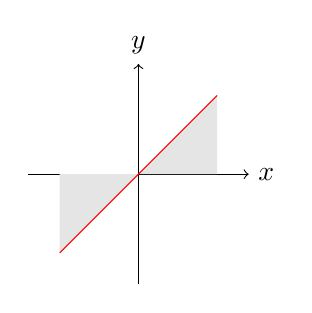
\begin{tikzpicture}
  \draw[->] (-1.4,0) -- (1.4,0) node[right] {$x$};
  \draw[->] (0,-1.4) -- (0,1.4) node[above] {$y$};
  \shade[top color=gray!20,bottom color=gray!20] 
      (0,0) (1,1) |- (0,0);
  \shade[top color=gray!20,bottom color=gray!20] 
      (-1,-1) |- (0,0) (-1,-1);
  \draw[scale=0.5,domain=-2:2,smooth,variable=\x,red] plot ({\x},{\x});
  %\draw[scale=0.5,domain=-3:3,smooth,variable=\y,red]  plot ({\y*\y},{\y});
\end{tikzpicture}
 \caption{St\"orung $H_1$}
 \label{abb:efeld_H_1}
\end{figure}

Allerdings wird durch die positive Spannung das Elektron angezogen und die
Wahrscheinlichkeit es weiter Rechts anzutreffen steigt.

Durch das elektrische Feld haben wir entlang der $x$-Achse verschieden Energie-Potentiale.
Das Elektron hat allerdings immer die selbe Energie,
die Energie muss sich also irgendwie ausgleichen.
Wir k"onnen diesen Vorgang einfach mit der Schr"odingergleichung verstehen:
\[
-\frac{\hbar^2}{2m}\Delta\Psi(x) + V(x)\Psi(x)
=
E \Psi(x)
\]
Weil $E \Psi(x)$ konstant ist, sinkt bei einem h"oherem Potential $-\frac{\hbar^2}{2m}\Delta\Psi(x)$.
Das bedeutet bei einem Elektron eine Abnahme der kinetischen Energie bzw. der Frequenz.
Der Vorgang ist also "ahnlich einem mechanischem Pendel, 
welches mal kinetische Energie hat, mal mechanische.

\begin{figure}
 \centering
 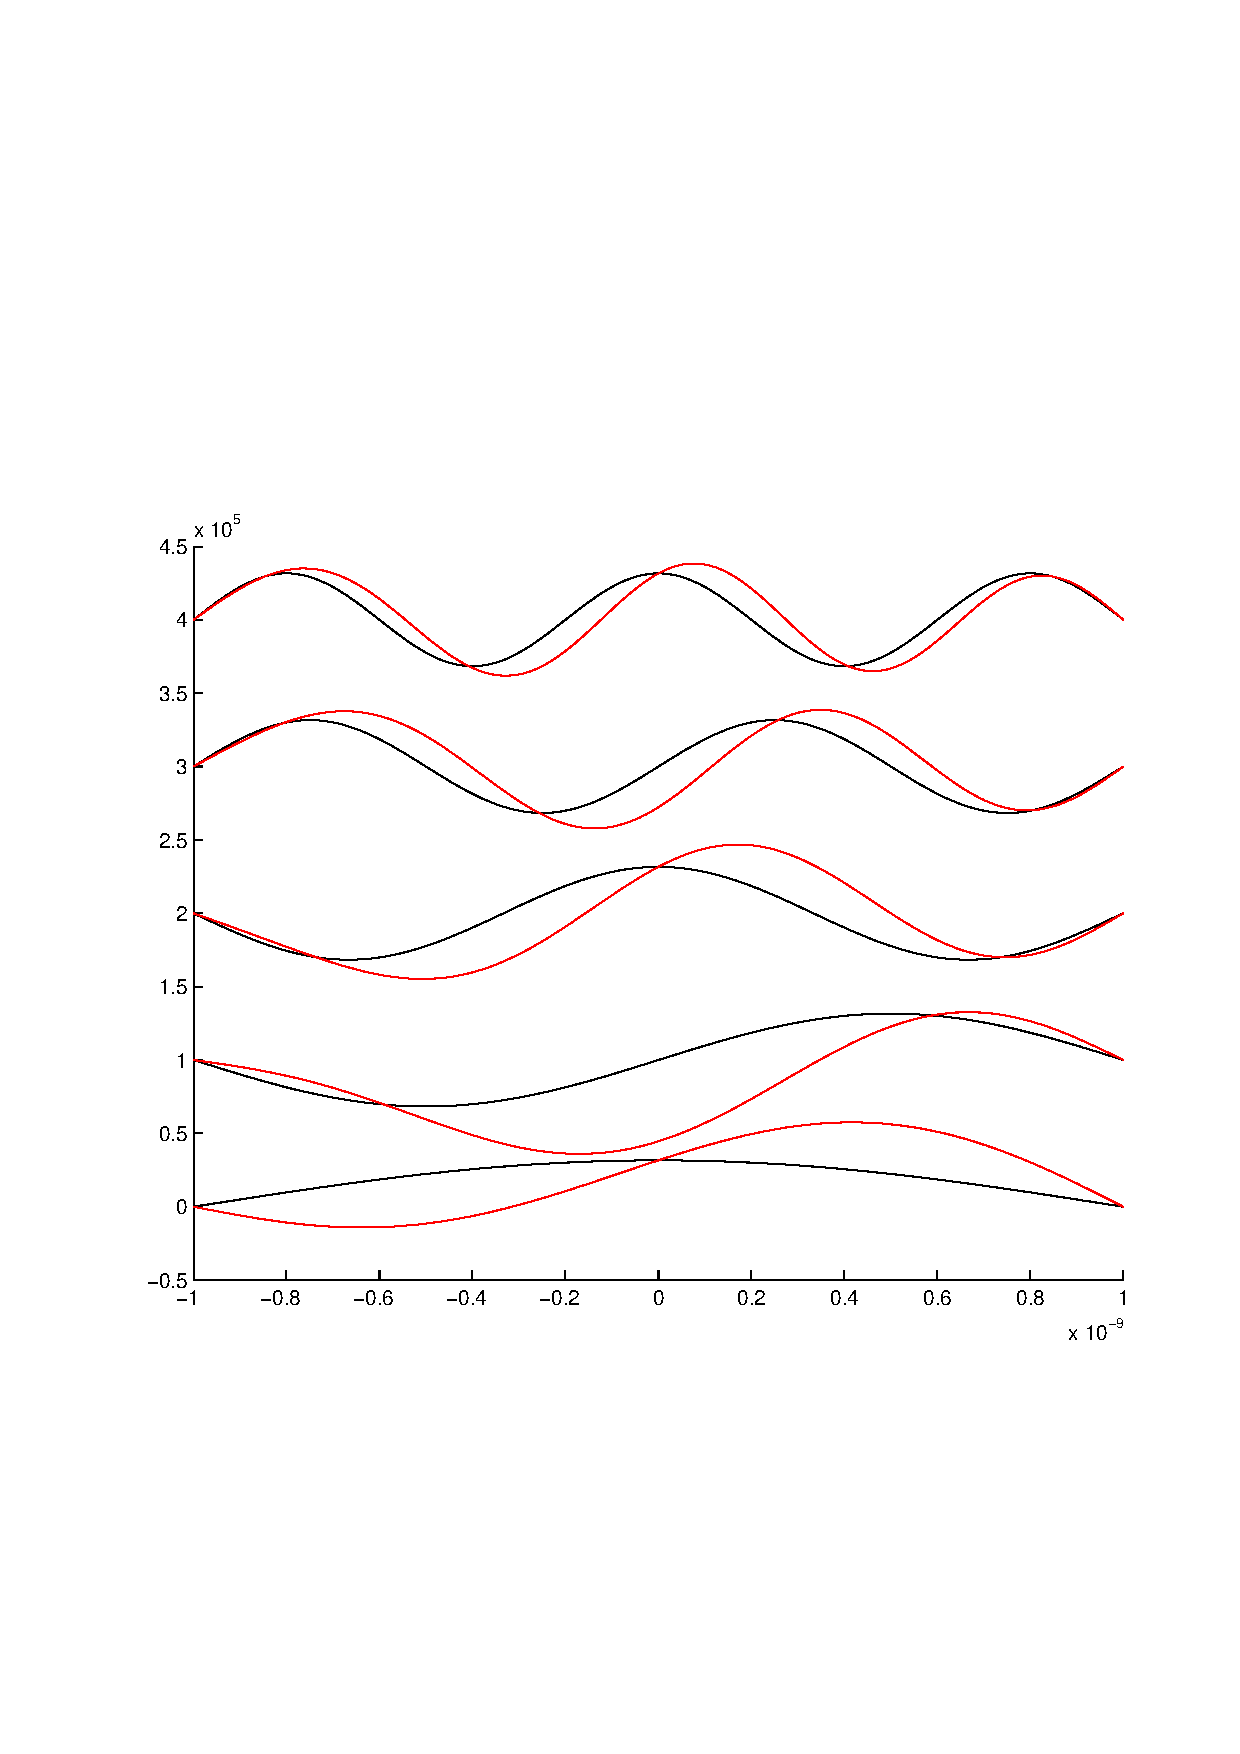
\includegraphics[width=12cm,clip=true,trim=2cm 7cm 1cm 8cm]{efeld/Psi_gestoert.pdf}
 \caption{$\psi$ gest\"ort}
 \label{abb:efeld_psi_gestoert}
\end{figure}



\subsection{Auswertung E}

Wie wir in der Berechnung festgestellt haben ver"andert sich der Energiezustand nicht.
H"atten wir eine Energie in der St"orung w"urde sie gegen oben immer schw"acher werden, weil $E_k^{(0)}$ immer gr"osser wird.

\begin{figure}
 \centering
 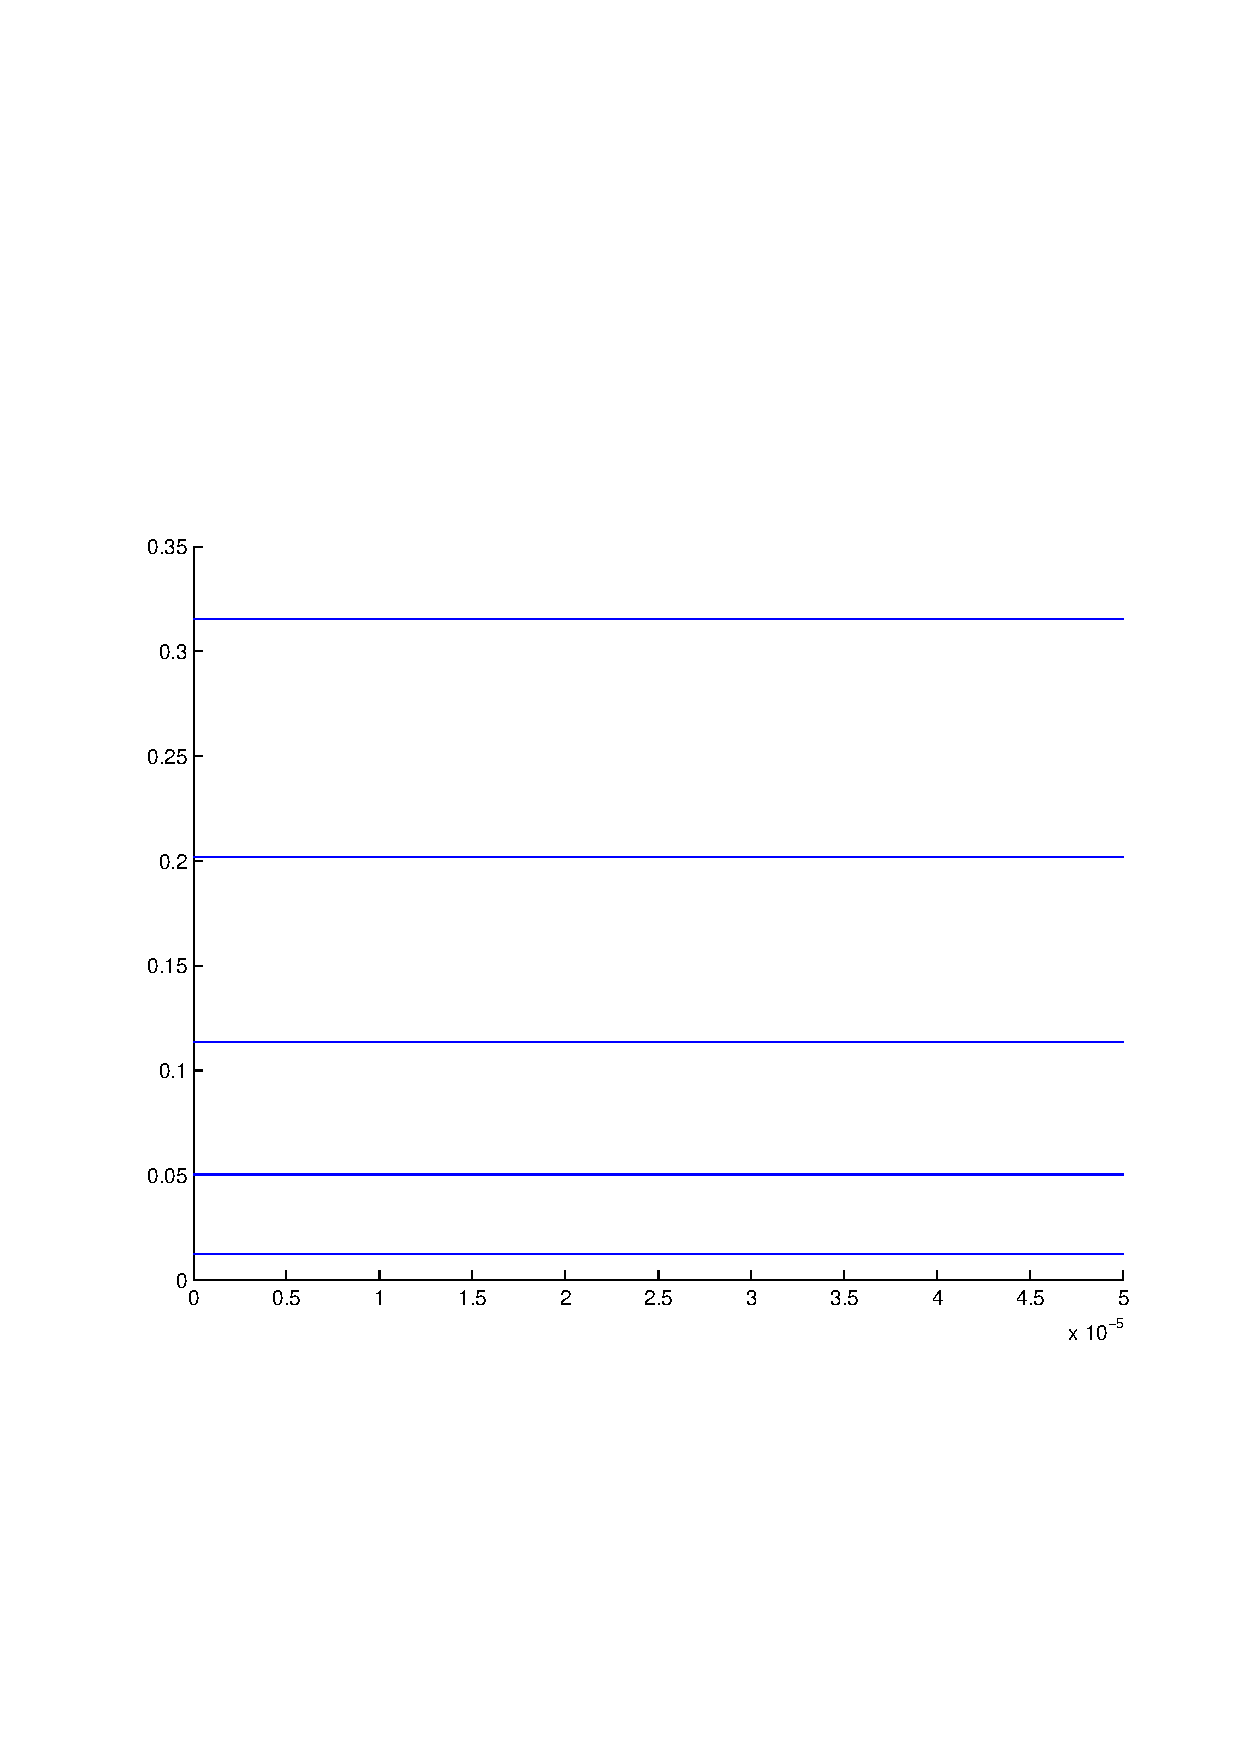
\includegraphics[width=12cm,clip=true,trim=2cm 7cm 1cm 8cm]{efeld/Energie_gestoert.pdf}
 \caption{$E$ gest\"ort, horizontale Achse ist $\varepsilon$, vertikale Achse ist die gesammte Energie des Systems}
 \label{abb:efeld_E_gestoert}
\end{figure}





\printbibliography[heading=subbibliography]
\end{refsection}
